\documentclass[../main.tex]{subfiles}






\begin{document}
\chapter{}
\label{cha:cha_15}

\section{}
\begin{enumerate}[label=\bfseries(\alph*)]
\item The simultaneous equations for the natural spline can be set up as
	\bigbreak
$
\left[\begin{array}{cccccc}
1 & & & & & \\
1 & 3 & 0.5 & & & \\
0.5 & 2 & 0.5 & & \\
& & 0.5 & 3 & 1 & \\
& & & 1 & 4 & 1 \\
& & & & & 1
\end{array}\right]\left\{\begin{array}{l}
c_{1} \\
c_{2} \\
c_{3} \\
c_{4} \\
c_{5} \\
c_{6}
\end{array}\right\}=\left\{\begin{array}{c}
0 \\
0 \\
-6 \\
-24 \\
15 \\
0
\end{array}\right\}
$
	\bigbreak
These equations can be solved for the c’s and then Eqs. (15.21) and (15.18) can be used to
solve for the b’s and the d’s. The coefficients for the intervals can be summarized as 
	\bigbreak
\begin{tabular}{ccccc}
interval&a&b&c&d\\
1&1&3.970954&0&0.029046\\
2&5&4.058091&0.087137&-0.40664\\
3&7&3.840249&-0.52282&-6.31535\\
4&8&-1.41909&-9.99585&5.414938\\
5&2&-5.16598&6.248963&-2.08299
\end{tabular}
	\bigbreak
These can be used to generate the following plot of the natural spline:
	\bigbreak
	\begin{figure}[H]
		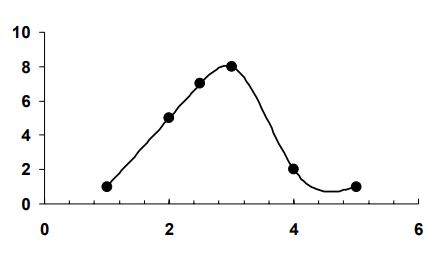
\includegraphics[width=0.5\linewidth]{fig_15_1}
		\label{fig:fig_15_1}
	\end{figure}
	\bigbreak
\item The not-a-knot spline and its plot can be generated with MATLAB as 
	\bigbreak
\begin{lstlisting}[numbers=none]
>> x = [1 2 2.5 3 4 5];
>> y = [1 5 7 8 2 1];
>> xx = linspace(1,5);
>> yy = spline(x,y,xx);
>> plot(x,y,'o',xx,yy)
\end{lstlisting}
	\bigbreak
	\begin{figure}[H]
		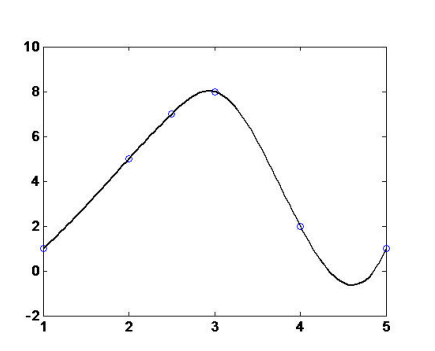
\includegraphics[width=0.5\linewidth]{fig_15_2}
		\label{fig:fig_15_2}
	\end{figure}
	\bigbreak
Notice how the not-a-knot version exhibits much more curvature, particularly between the
last points
	\bigbreak
\item 
The piecewise cubic Hermite polynomial and its plot can be generated with MATLAB as
	\bigbreak
\begin{lstlisting}[numbers=none]
>> x = [1 2 2.5 3 4 5];
>> y = [1 5 7 8 2 1];
>> xx = linspace(1,5);
>> yy = interp1(x,y,xx,'pchip');
>> plot(x,y,'o',xx,yy)
\end{lstlisting}
	\bigbreak
	\begin{figure}[H]
		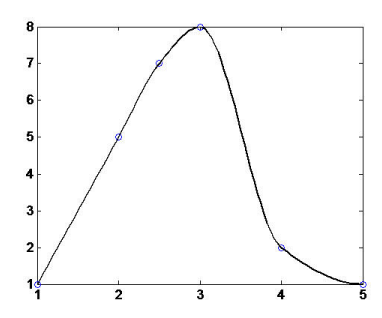
\includegraphics[width=0.5\linewidth]{fig_15_3}
		\label{fig:fig_15_3}
	\end{figure}
	\bigbreak



\section{}
The simultaneous equations for the clamped spline with zero end slopes can be set up as 
	\bigbreak
$
\left[\begin{array}{ccccccc}
1 & 0.5 & & & & & \\
0.5 & 2 & 0.5 & & & & \\
& 0.5 & 2 & 0.5 & & & \\
& & 0.5 & 2 & 0.5 & & \\
& & & 0.5 & 2 & 0.5 & \\
& & & & 0.5 & 2 & 0.5 \\
& & & & & 0.5 & 1
\end{array}\right]\left\{\begin{array}{c}
c_{1} \\
c_{2} \\
c_{3} \\
c_{4} \\
c_{5} \\
c_{6} \\
c_{7}
\end{array}\right\}=\left\{\begin{array}{c}
0 \\
-90 \\
-108 \\
144 \\
36 \\
18 \\
 \\
\end{array}\right\}
$
	\bigbreak
These equations can be solved for the c’s and then Eqs. (15.21) and (15.18) can be used to
solve for the b’s and the d’s. The coefficients for the intervals can be summarized as
	\bigbreak
\begin{tabular}{ccccc}
interval&a&b&c&d\\
1&70&0&15.87692&-31.7538\\
2&70&-7.93846&-31.7538&-24.7385\\
3&55&-58.2462&-68.8615&106.7077\\
4&22&-47.0769&91.2&-66.0923\\
5&13&-5.44615&-7.93846&13.66154\\
6&10&-3.13846&12.55385&-12.5538
\end{tabular}
	\bigbreak
The fit can be displayed in graphical form. Note that we are plotting the points as depth
versus temperature so that the graph depicts how the temperature changes down through the
tank. 
	\bigbreak
	\begin{figure}[H]
		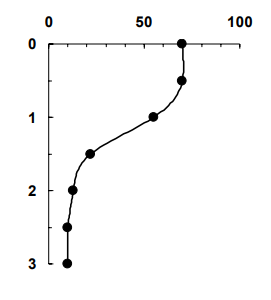
\includegraphics[width=0.5\linewidth]{fig_15_4}
		\label{fig:fig_15_4}
	\end{figure}
	\bigbreak
Inspection of the plot indicates that the inflection point occurs in the $3^{\text {rd }}$ interval. The cubic equation for this interval is
	\bigbreak
$T_{3}(x)=55-58.2462(d-1)-68.8615(d-1)^{2}+106.7077(d-1)^{3}$
	\bigbreak
where T = temperature and d = depth. This equation can be differentiated twice to yield the
second derivative
	\bigbreak
$\dfrac{d^{2} T_{3}(x)}{d x^{2}}=-137.729+640.2462(d-1)$
	\bigbreak
This can be set equal to zero and solved for the depth of the thermocline as d = 1.21511 m.
	\bigbreak
\end{enumerate}


\section{}
\begin{enumerate}[label=\bfseries(\alph*)]
\item The not-a-knot fit can be set up in MATLAB as
\begin{lstlisting}[numbers=none]
>> x = linspace(0,1,11);
>> y = 1./((x-0.3).^2+0.01)+1./((x-0.9).^2+0.04)-6;
>> xx = linspace(0,1);
>> yy = spline(x,y,xx);
>> yh = 1./((xx-0.3).^2+0.01)+1./((xx-0.9).^2+0.04)-6;
>> plot(x,y,'o',xx,yy,xx,yh,'--') 
\end{lstlisting}
	\bigbreak
	\begin{figure}[H]
		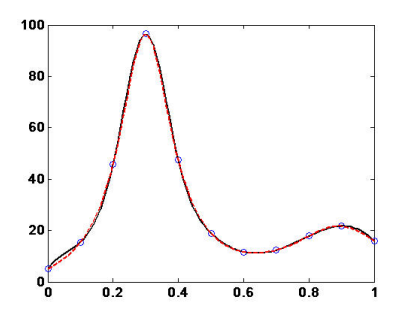
\includegraphics[width=0.5\linewidth]{fig_15_5}
		\label{fig:fig_15_5}
	\end{figure}
	\bigbreak
\item The piecewise cubic Hermite polynomial fit can be set up in MATLAB as 
	\bigbreak
\begin{lstlisting}[numbers=none]
>> x = linspace(0,1,11);
>> y = 1./((x-0.3).^2+0.01)+1./((x-0.9).^2+0.04)-6;
>> xx = linspace(0,1);
>> yy = interp1(x,y,xx,'pchip');
>> yh = 1./((xx-0.3).^2+0.01)+1./((xx-0.9).^2+0.04)-6;
>> plot(x,y,'o',xx,yy,xx,yh,'--')
\end{lstlisting}
	\begin{figure}[H]
		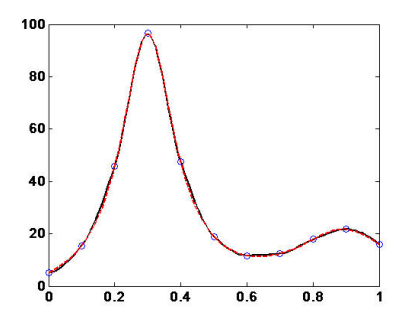
\includegraphics[width=0.5\linewidth]{fig_15_6}
		\label{fig:fig_15_6}
	\end{figure}
	\bigbreak
\end{enumerate}



\section{}
\begin{enumerate}[label=\bfseries(\alph*)]
\item The simultaneous equations for the clamped spline with zero end slopes can be set up as 
	\bigbreak
$
\left[\begin{array}{ccccccc}
1 & & & & & \\
100 & 400 & 100 & & & & \\
100 & 600 & 200 & & & \\
c_{3} \\
c_{4} \\
c_{5} \\
c_{6} \\
c_{7}
\end{array}\right\}=\left\{\begin{array}{l}
c_{1} \\
-0.01946 \\
-0.00923 \\
-0.00098 \\
0.001843 \\
0.001489 \\
0
\end{array}\right\}
$
	\bigbreak
These equations can be solved for the c’s and then Eqs. (15.21) and (15.18) can be used to
solve for the b’s and the d’s. The coefficients for the intervals can be summarized as
	\bigbreak
\begin{tabular}{ccccc}
interval&a&b&c&d\\
1&0&0.009801&0&-1.6E-07\\
2&0.824361&0.005128&-4.7E-05&1.3E-07\\
3&1&-0.00031&-7.7E-06&1.31E-08\\
4&0.735759&-0.0018&2.13E-07&2.82E-09\\
5&0.406006&-0.00138&1.9E-06&-8.7E-10\\
6&0.199148&-0.00072&1.39E-06&-2.3E-09
\end{tabular}
	\bigbreak
The fit can be displayed in graphical form as
	\bigbreak
	\begin{figure}[H]
		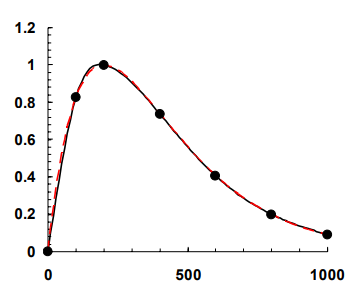
\includegraphics[width=0.5\linewidth]{fig_15_7}
		\label{fig:fig_15_7}
	\end{figure}
	\bigbreak
\item The not-a-knot fit can be set up in MATLAB as
	\bigbreak
\begin{lstlisting}[numbers=none]
>> x = [0 100 200 400 600 800 1000];
>> y = x/200.*exp(-x/200+1);
>> xx = linspace(0,1000);
>> yc = xx/200.*exp(-xx/200+1);
>> yy = spline(x,y,xx);
>> plot(x,y,'o',xx,yy,xx,yc,'--') 
\end{lstlisting}
	\bigbreak
	\begin{figure}[H]
		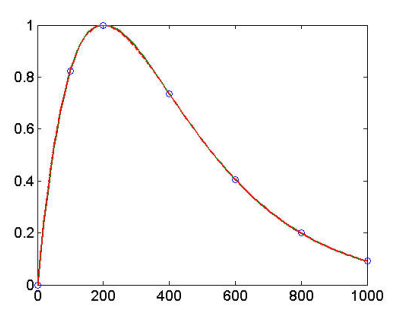
\includegraphics[width=0.5\linewidth]{fig_15_8}
		\label{fig:fig_15_8}
	\end{figure}
	\bigbreak
\item The piecewise cubic Hermite polynomial fit can be set up in MATLAB as
	\bigbreak
\begin{lstlisting}[numbers=none]
>> x = [0 100 200 400 600 800 1000];
>> y = x/200.*exp(-x/200+1);
>> xx = linspace(0,1000);
>> yc = xx/200.*exp(-xx/200+1);
>> yy = interp1(x,y,xx,'pchip');
>> plot(x,y,'o',xx,yy,xx,yc,'--') 
\end{lstlisting}
	\bigbreak
	\begin{figure}[H]
		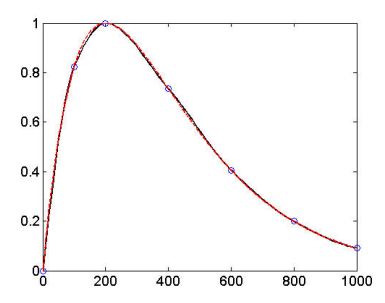
\includegraphics[width=0.5\linewidth]{fig_15_9}
		\label{fig:fig_15_9}
	\end{figure}
	\bigbreak
Summary: For this case, the not-a-knot fit is the best.
	\bigbreak
\end{enumerate}



\section{}
\begin{enumerate}[label=\bfseries(\alph*)]
\item The not-a-knot fit can be set up in MATLAB as
	\bigbreak
\begin{lstlisting}[numbers=none]
>> x = [-1 -0.6 -0.2 0.2 0.6 1];
>> y = [0 0 0 1 1 1];
>> xx = linspace(-1,1);
>> yy = spline(x,y,xx);
>> plot(x,y,'o',xx,yy) 
\end{lstlisting}
	\bigbreak
	\begin{figure}[H]
		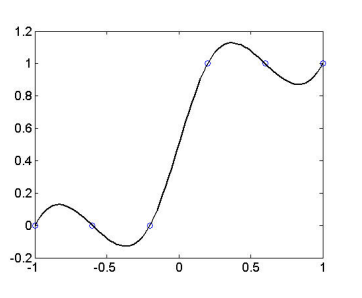
\includegraphics[width=0.5\linewidth]{fig_15_10}
		\label{fig:fig_15_10}
	\end{figure}
	\bigbreak
\item The clamped spline with zero end slopes can be set up in MATLAB as
	\bigbreak
\begin{lstlisting}[numbers=none]
>> x = [-1 -0.6 -0.2 0.2 0.6 1];
>> y = [0 0 0 1 1 1];
>> ys = [0 y 0];
>> xx = linspace(-1,1);
>> yy = spline(x,ys,xx);
>> plot(x,y,'o',xx,yy) 
\end{lstlisting}
	\bigbreak
	\begin{figure}[H]
		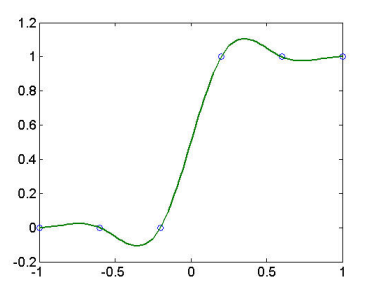
\includegraphics[width=0.5\linewidth]{fig_15_11}
		\label{fig:fig_15_11}
	\end{figure}
	\bigbreak
\item The piecewise cubic Hermite polynomial fit can be set up in MATLAB as
	\bigbreak
\begin{lstlisting}[numbers=none]
>> x = [-1 -0.6 -0.2 0.2 0.6 1];
>> y = [0 0 0 1 1 1];
>> xx = linspace(-1,1);
>> yy = interp1(x,y,xx,'pchip');
>> plot(x,y,'o',xx,yy) 
\end{lstlisting}
	\bigbreak
	\begin{figure}[H]
		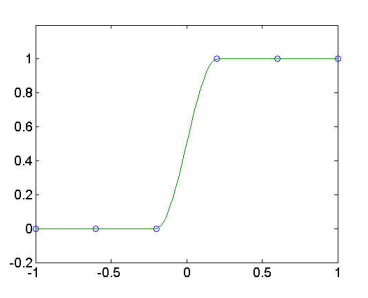
\includegraphics[width=0.5\linewidth]{fig_15_12}
		\label{fig:fig_15_12}
	\end{figure}
	\bigbreak
\end{enumerate}



\section{}
An M-file function to implement the natural spline can be written as
\begin{lstlisting}[numbers=none]
function yy = natspline(x,y,xx)
% natspline(x,y,xx):
% uses a natural cubic spline interpolation to find yy, the values
% of the underlying function y at the points in the vector xx.
% The vector x specifies the points at which the data y is given.


n = length(x);
m = length(xx);
aa(1,1) = 1; aa(n,n) = 1;
bb(1) = 0; bb(n) = 0;
for i = 2:n-1
	aa(i,i-1) = h(x, i - 1);
	aa(i,i) = 2 * (h(x, i - 1) + h(x, i));
	aa(i,i+1) = h(x, i);
	bb(i) = 3 * (fd(i + 1, i, x, y) - fd(i, i - 1, x, y));
end
c = aa\bb';
for i = 1:n - 1
	a(i) = y(i);
	b(i) = fd(i + 1, i, x, y) - h(x, i) / 3 * (2 * c(i) + c(i + 1));
	d(i) = (c(i + 1) - c(i)) / 3 / h(x, i);
end
for i = 1:m
	yy(i) = SplineInterp(x, n, a, b, c, d, xx(i));
end


function hh = h(x, i)
hh = x(i + 1) - x(i);


function fdd = fd(i, j, x, y)
fdd = (y(i) - y(j)) / (x(i) - x(j));


function yyy = SplineInterp(x, n, a, b, c, d, xi)
for ii = 1:n - 1
	if xi >= x(ii) - 0.000001 & xi <= x(ii + 1) + 0.000001
		yyy=a(ii)+b(ii)*(xi-x(ii))+c(ii)*(xi-x(ii))^2+d(ii)*(xi-x(ii))^3;
		break
	end
end 
\end{lstlisting}
	\bigbreak
The program can be used to duplicate Example 15.3:
	\bigbreak
\begin{lstlisting}[numbers=none]
>> x = [3 4.5 7 9];
>> y = [2.5 1 2.5 .5];
>> xx = linspace(3,9);
>> yy = natspline(x,y,xx);
>> plot(x,y,'o',xx,yy) 
\end{lstlisting}
	\begin{figure}[H]
		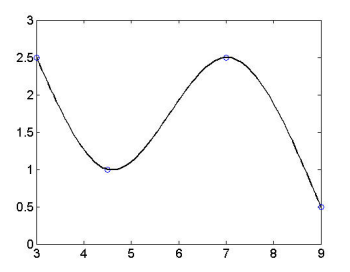
\includegraphics[width=0.5\linewidth]{fig_15_13}
		\label{fig:fig_15_13}
	\end{figure}
	\bigbreak



\section{}
\begin{enumerate}[label=\bfseries(\alph*)]
\item The not-a-knot fit can be set up in MATLAB as
	\bigbreak
\begin{lstlisting}[numbers=none]
>> x = [1 3 5 6 7 9];
>> y = 0.0185*x.^5-0.444*x.^4+3.9125*x.^3-15.456*x.^2+27.069*x-14.1;
>> xx = linspace(1,9);
>> yy = spline(x,y,xx);
>> yc = 0.0185*xx.^5-0.444*xx.^4+3.9125*xx.^3-15.456*xx.^2+27.069*xx-14.1;
>> plot(x,y,'o',xx,yy,xx,yc,'--') 
\end{lstlisting}
	\begin{figure}[H]
		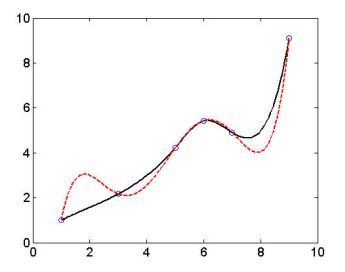
\includegraphics[width=0.5\linewidth]{fig_15_14}
		\label{fig:fig_15_14}
	\end{figure}
	\bigbreak
\item The function can be differentiated to give
	\bigbreak
$f^{\prime}(x)=0.0925 x^{4}-1.776 x^{3}+11.7375 x^{2}-30.912 x+27.069$
	\bigbreak
This function can be evaluated at the end nodes to give $f^{\prime}(1)=6.211$ and $f(9)=11.787$. These values can then be added to the $y$ vector and the spline function invoked to develop the clamped fit:
	\bigbreak
\begin{lstlisting}[numbers=none]
>> yd = [6.211 y 11.787];
>> yy = spline(x,yd,xx);
>> plot(x,y,'o',xx,yy,xx,yc,'--') 
\end{lstlisting}
	\begin{figure}[H]
		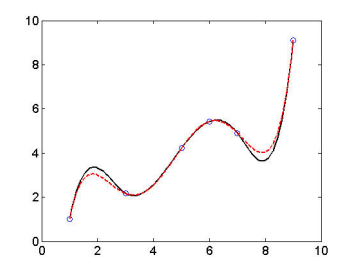
\includegraphics[width=0.5\linewidth]{fig_15_15}
		\label{fig:fig_15_15}
	\end{figure}
	\bigbreak
\end{enumerate}
\end{document}